\section{Coordinated MAB}
\label{sec:solution}

We consider a Multi-Agent MAB (MA-MAB) setting in which multiple agents are individually enrolled in different BSSs for optimizing SR by tuning the PD (which determines to which extent inter-BSS interference can be ignored) and the transmit power (which determines to which extent inter-BSS interference is created). The proposed solution departs from the operations defined for OBSS/PD-based SR, which was detailed in~\cite{wilhelmi2021spatial}, hence making it compatible with currently available products. As a step further, and by leveraging MAPC capabilities, we allow agents to exchange feedback about their performance regularly, thus aiming at creating collaborative strategies that enhance global performance. Formally, based on some action--selection strategy $\mathcal{E}$ (cf. Section~\ref{sec:action_selection}), each player (or agent) $p\in \mathcal{P}$ sequentially plays an action (or arm) $k\in \mathcal{A}^{(p)}$ at each time step $t=1,...,T$ and obtains a reward $r^{(p)}(t+1) \in \mathbb{R}$ that depends on the joint action profile $K(t)= \{k^{(1)}(t), ..., k^{(|\mathcal{P}|)}(t)\}$ and on the reward calculation strategy $\mathcal{R}$ (cf. Section~\ref{sec:reward_calculation}). For the SR problem, we consider actions composed of discrete PD ($\gamma$) and transmit power ($\zeta$) values, which leads to an individual action space $\mathcal{A}^{(p)}_{|\gamma|\times|\zeta|}$ and a global action space $\mathcal{A}_{|\mathcal{P}|\times|\gamma|\times |\zeta|}$.

\begin{figure}[ht!]
    \centering
    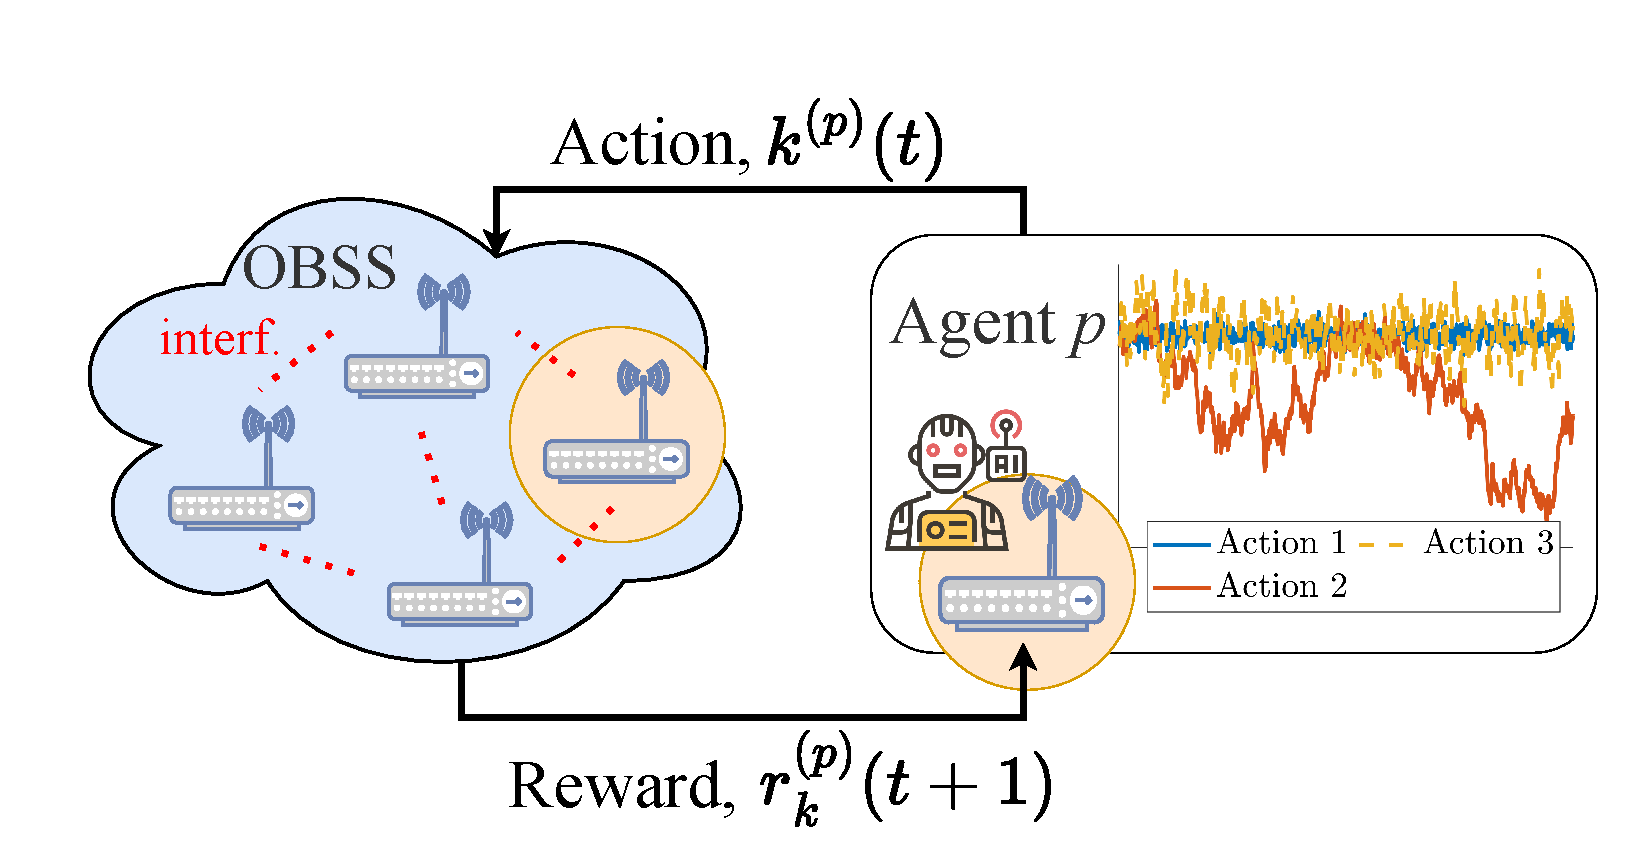
\includegraphics[width=0.8\columnwidth]{figures/agents_operation.pdf}
    \caption{Representation of an agent's operation in an OBSS, where the rewards associated with the different available actions are drawn from an unknown distribution.}
    \label{fig:agents_operation}
\end{figure}

MAB operation is illustrated in Figure~\ref{fig:agents_operation} and is generically described in Algorithm~\ref{alg:bandit}. After initializing the rewards $r_k^{(p)}$ and the number of plays $N_k^{(p)}$ for each action $k\in \mathcal{A}^{(p)}$, agent $p$ sequentially selects an action based on the action-selection strategy $\mathcal{E}$ (line~4 in Algorithm~\ref{alg:bandit}) and, in the next iteration, receives a reward based on the reward calculation strategy $\mathcal{R}$ (line~3 in Algorithm~\ref{alg:bandit}). The simultaneous operation of multiple agents breaks the stationarity of the rewards' distributions, thus making the problem challenging. Nevertheless, the multi-agent setting keeps the complexity of the problem low, which otherwise would lead to a combinatorial action space.

\begin{algorithm}[h!]
	\SetKwInOut{Input}{Input}
	\SetKwInOut{Output}{Output}		
	\textbf{Initialize:} $t=0$, for each arm $k \in \mathcal{A}^{(p)}$, set $r^{(p)}_{k} = 0$ and $N^{(p)}_k = 0$ \\
	\For{$t = 1...T$}
	{
         Update the reward $r_{k}(t)$ based on the performance observed in $t+1$ and $\mathcal{R}$ \\
         Select arm $k\in \mathcal{A}^{(p)}$ based on $\mathcal{E}$\\
         $N^{(p)}_{k} \leftarrow N^{(p)}_{k} + 1$\\
	}
	\caption{MAB implementation by agent $p$.}
	\label{alg:bandit}
\end{algorithm}	

\subsection{Action Selection Strategy ($\mathcal{E}$)}
\label{sec:action_selection}

We focus on two exploration--exploitation strategies, namely $\varepsilon$-greedy~\cite{auer2002finite} and Thompson sampling~\cite{thompson1933likelihood}, for driving the training of agents towards finding the best actions. First, $\varepsilon$-greedy is a classic strategy used in reinforcement learning whereby an agent samples an arm uniformly at random ($\mathcal{U}$) with a certain fixed probability (exploration) and selects the arm yielding the best-observed performance the rest of the time (exploitation). The $\varepsilon$-greedy algorithm, despite its simplicity, has been shown to be effective in complex settings such as OBSS~\cite{barrachina2021multi}. In particular, an agent implementing $\varepsilon$-greedy selects an arm as:
\begin{equation}
    k=\begin{cases}      
    k \sim \mathcal{U}(1, |\mathcal{A}^{(p)}|), & \text{with prob. } \varepsilon~ \text{(exploration)}, \\ 
    \underset{k\in\mathcal{A}^{(p)}}{\text{argmax }} r^{(p)}_{k}, & \text{with prob. } 1 - \varepsilon~\text{(exploitation)}.
    \end{cases}
\end{equation}

Thompson sampling addresses exploration-exploitation in a different way than $\varepsilon$-greedy: that it samples arms based on their probability of being optimal, according to a probabilistic model constructed from the observed rewards. In particular, as previously done in \cite{wilhelmi2019potential}, we assume that the distribution of the reward associated with each arm is given by a Gaussian distribution $\mathcal{N}$. Based on that, an agent implementing Thompson sampling selects, in each iteration, the arm maximizing $\text{argmax }_{k\in\mathcal{A}^{(p)}} \theta_k$, where
\begin{equation}
    \theta_{k\in\mathcal{A}^{(p)}}\sim \mathcal{N}\bigg(\hat{r}_{k}^{(p)}, \frac{1}{N_k^{(p)} + 1}\bigg),
\end{equation}
where the estimated reward $\hat{r}_{k}^{(p)}$ is given by
\begin{equation}
    \hat{r}_{k}^{(p)} \leftarrow \frac{\hat{r}_{k}^{(p)}  N^{(p)}_{k} + r^{(p)}_{k}}{r^{(p)}_{k} + 2}.
\end{equation}

\subsection{Reward Calculation Strategy ($\mathcal{R}$)}
\label{sec:reward_calculation}

To compute the reward, we consider different sharing strategies, which are based on a selfish reward (\texttt{SELF}) that is firstly computed by each agent individually. In particular, the selfish reward is calculated as the normalized individual throughput $r^{(p)}=\Gamma^{(p)}/\Gamma^{*(p)}$, where $\Gamma^{*(p)}$ is the maximum achievable throughput in isolation, derived from the maximum transmission capabilities of the BSS given by the best applicable Modulation and Coding Scheme (MCS).\footnote{Other performance indicators such as latency can be adopted as a reward.} As for the sharing strategies, enabled by the MAPC framework, they allow the different agents to play actions according to a shared performance among the players. From the MAB algorithms' perspective, MAPC is assumed to allow for a perfect monitoring setting, which means that every agent has access to the rewards experienced by others. According to this, we study the following shared reward criteria:
\begin{itemize}
    \item \textbf{Average, \texttt{AVG}:} The shared reward is calculated as the average value of each individual reward, so that $r_\texttt{AVG} = \frac{1}{|\mathcal{P}|}\sum_{p=1}^{|\mathcal{P}|} r^{(p)}$.
    \item \textbf{Max-min, \texttt{MAX-MIN}:} The shared reward is computed as the minimum value of each individual reward, so that $r_\texttt{MAX-MIN} = \min_{p\in \mathcal{P}} (r^{(p)})$.
    \item \textbf{Proportional fairness, \texttt{PF}:} The shared reward is calculated as the sum of the logarithms of each individual reward, so that $r_\texttt{PF} = \sum_{p=1}^{|\mathcal{P}|} \log(r^{(p)})$.
\end{itemize}

In this work, we assume that the communication between agents for sharing the rewards is negligible and lossless, and occurs at the end of each learning iteration of fixed duration $\Delta$. Future work is expected to shed light on the overheads associated with the coordinated MABs, as well as on the implications of sharing information through wireless links exposed to contention and interference effects.
